\textbf{$\ket{+} = \frac{1}{\sqrt{2}}(\ket{0}+\ket{1})$}\vspace{.2cm}

\textcolor{bibi}{Por definición}\vspace{.2cm}
\begin{quote}
    \begin{minted}[fontsize=\small, linenos, frame=single]{python}
circuitoMas = QuantumCircuit(1)
circuitoMas.h(0)
circuitoMas.measure_all()
circuitoMas.draw('mpl')
    \end{minted}
    \vspace{.3cm}
    \begin{center}
        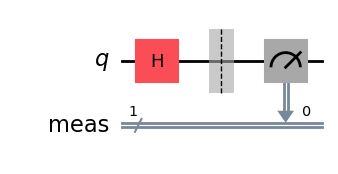
\includegraphics[height=3.3cm]{src/Img/1.2.png}
    \end{center}

    Este es un poquito mas complicado pero sale de la propiedad de que
    $\hat{H}\ket{0}=\ket{+}$ y como nuestros \texttt{qubits} se inicializan en 0 por
    defecto, solo es aplicar la compuerta H. Si la medimos nos queda así:
    \vspace{.5cm}

    \begin{center}
        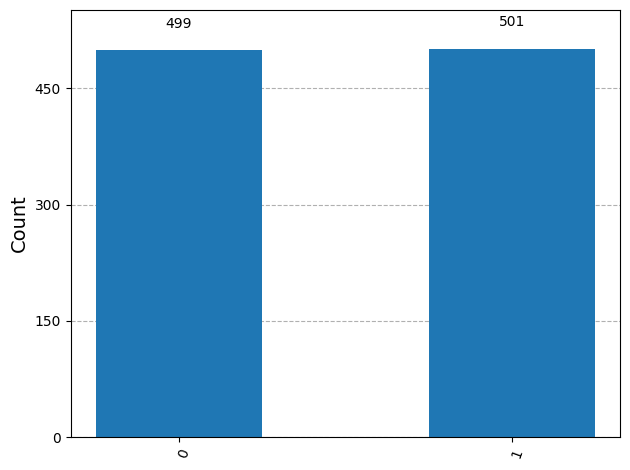
\includegraphics[height=6cm]{src/Img/1.2.r.png}
    \end{center}
\end{quote}
\vspace{.4cm}
